\documentclass[a4paper,slidestop,xcolor=pst,blue]{beamer}

\usepackage{beamerthemesplit}
\usepackage[utf8]{inputenc}
\usepackage[spanish]{babel}
\usepackage{graphicx}
\usepackage{pstricks} % PSTricks package
\usepackage{setspace}
\usepackage{multirow}
\usepackage{listings}
\usepackage{pgfpages}
\usepackage{hyperref}
\usepackage{etoolbox}
\usepackage{epstopdf}

\makeatletter
\patchcmd{\beamer@sectionintoc}{\vskip1.5em}{\vskip0.5em}{}{}
\makeatother

\setbeamercovered{dynamic}
\setcounter{tocdepth}{2}
\setbeamercolor{frametitle}{fg=black,bg=white}
\setbeamercolor{section in toc shaded}{fg=black}
\setbeamercolor{section in toc}{fg=red}
\setbeamercolor{subsection in toc shaded}{fg=black}
\setbeamercolor{subsection in toc}{fg=red}
\setbeamerfont{section in toc}{size=\small}
\setbeamerfont{subsection in toc}{size=\small}
\setbeamertemplate{section in toc shaded}[default][99]
\setbeamertemplate{subsection in toc shaded}[default][99]

\AtBeginSection[]
{\begin{frame}[c]
  \frametitle{Índice}
	\tableofcontents[currentsection,
        sectionstyle=show/shaded,
        subsectionstyle=hide]
\end{frame}}

\AtBeginSubsection[]
{\begin{frame}[c]
	\frametitle{Índice}
	\tableofcontents[
  		currentsection,
  		sectionstyle=shaded/shaded,
  		currentsubsection,
  		subsectionstyle=show/shaded/hide
		]
\end{frame}}

\setbeamercolor{frametitle}{fg=black,bg=white}

\setbeamertemplate{frametitle}{
	\begin{centering}
		\insertframetitle
		\par
	\end{centering}
}

\usetheme[secheader]{Boadilla} 

\usepackage{pifont}
\newcommand{\cmark}{\ding{51}}
\newcommand{\xmark}{\ding{55}}

\title[Spring Data + JPA]{Capa de Persistencia \\ \ \\ Spring Data + Java Persistence API (JPA)}

\author[P. S{\'a}nchez]{\alert{Pablo S{\'a}nchez}}

\institute[IIE]{
		   Dpto. Ingenier{\'i}a Inform{\'a}tica y Electr{\'o}nica \\
		   Universidad de Cantabria \\
		   Santander (Cantabria, Espa{\~n}a) \\
		   \texttt{p.sanchez@unican.es}
}

\date{}

\begin{document}

\begin{frame}[c]
	\titlepage
	\begin{columns}
		\column{0.50\linewidth}
			\centering
    		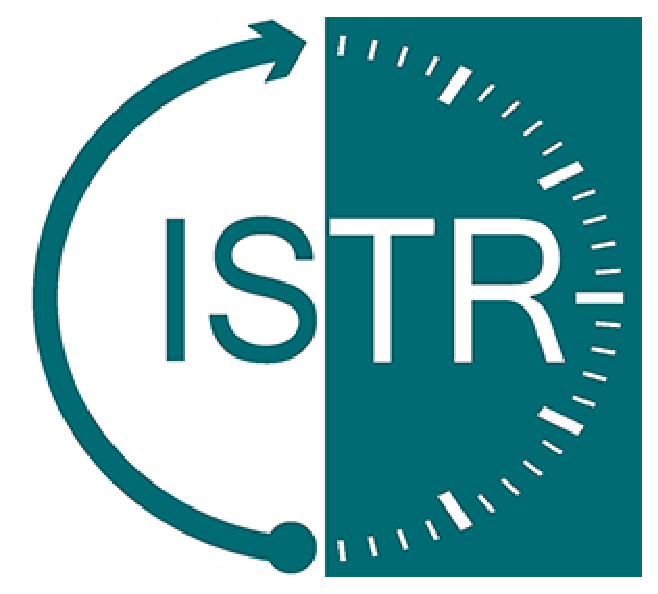
\includegraphics[width=.28\textwidth,keepaspectratio=true]{images/istr.eps}
		\column{0.50\linewidth}
			\centering
			
\includegraphics[width=.25\textwidth,keepaspectratio=true]{images/uc.eps}
	\end{columns}
\end{frame}

\begin{frame}[c]
    \frametitle{\alert{Advertencia}}
    \begin{center}
        Todo el material contenido en este documento no constituye en modo alguno una obra de referencia o apuntes oficiales mediante el cual se puedan preparar las pruebas evaluables necesarias para superar la asignatura. \ \\
        \ \\
        Este documento contiene exclusivamente una serie de diapositivas cuyo objetivo es servir de complemento visual a las actividades realizadas en el aula para la transmisi{\'o}n del contenido sobre el cual versar{\'a}n las mencionadas pruebas evaluables.  \ \\
        \ \\
        Dicho de forma m{\'a}s clara, \alert{estas transparencias no son apuntes y su objetivo no es servir para que el alumno pueda preparar la asignatura.}
    \end{center}
\end{frame}

\section{Introducción}

\begin{frame}
    \frametitle{Puentes de Persistencia de Objetos}
        \rput[lt](0,0){
            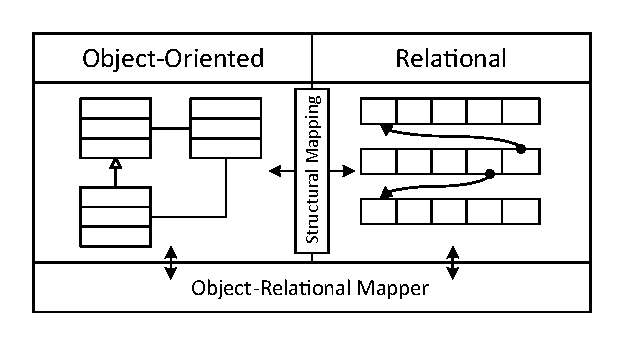
\includegraphics[width=\linewidth]{images/introduction/orm02.eps}
        }
    }
\end{frame}

\begin{frame}[c]
    \frametitle{JPA + Spring Data}
    \begin{block}{JPA}
        \begin{enumerate}
            \item \emph{Java Persistence API (JPA)} es una especificación estándar o interfaz de cómo realizar un puente de persistencia en Java.
            \item<2-> Proporciona dos maneras concretas (anotaciones y fichero externo XML) de especificar un \emph{metadata mapping}.
            \item<3-> Especifica la interfaz y funcionamiento de una serie de elementos para realizar el acceso a datos (e.g. \emph{PesistenceContext}).
            \item<4-> Precisan de un ORM que la implemente (e.g. Hibernate, Spring).
        \end{enumerate}
    \end{block}
    \uncover<5->{
        \begin{block}{Spring Data}
            Framework que proporciona facilidades para la definición de repositorios compatible con diversas tecnologías y de persistencia, entre ellas JPA.
        \end{block}
    }
\end{frame}

\begin{frame}[c]
    \frametitle{Objetivos del Tema}
    \begin{enumerate}[<+->]
         \item Ser capaz de transformar un conjunto de POJOs en un esquema relacional usando anotaciones JPA.
         \item Ser capaz crear repositorios JPA y \emph{Spring}.
         \item Ser capaz de utilizar repositorios Spring para interactuar con la capa de persistencia.
    \end{enumerate}
\end{frame}

\begin{frame}[c]
    \frametitle{Bibliografía}
    \begin{thebibliography}{1}

        \bibitem[Bauer, 2015]{Bauer2015}
        Bauer, C., King. G. y Gregory G. (2015).
        \newblock {\em {Java Persistence with Hibernate}}. 2ª Ed.
        \newblock Manning

        %% Spring Data

    \end{thebibliography}
\end{frame}

\section{Anotaciones JPA}

\begin{frame}[c]
    \frametitle{Entidades y Value Objects}
    \begin{description}
        \item[@Entity] Indica que un elemento es una entidad y se transformará a su correspondiente tabla.
        \item[@Embeddable] Indica que un elemento es un \emph{value object} y por tanto puede ser incrustado dentro de otro objeto.
    \end{description}
\end{frame}

\begin{frame}[c]
    \frametitle{Identificación de Entidades}
    \begin{description}
        \item[@Id] Especifica que un atributo de la clase ejerce de clave primaria.
        \item[@GeneratedValue] Indica que se desea que una clave artificial sea autogenerada.
        \item[@IdClass,@EmbeededId] Permite la creación de claves compuestas por varios campos.
    \end{description}
\end{frame}

\begin{frame}[c]
    \frametitle{Transformación de Asociaciones}
    \begin{description}
        \item[@OneToOne]
        \item[@OneToMany]
        \item[@ManyToOne]
        \item[@ManyToMany]
        \item[@Embedded]
        \item[@ElementsCollection]
        \item[mappeddBy]
    \end{description}
\end{frame}

\begin{frame}[c]
    \frametitle{Transformación de Herencias}
    \begin{description}
        \item[@@Inheritance(strategy=)]
        \item[@DiscriminatorValue]
    \end{description}
\end{frame}

\begin{frame}[c]
    \frametitle{Personalización de Elementos}
    \begin{description}
        \item[@Table]
        \item[@Column]
        \item[@JoinColumn]
        \item
    \end{description}
\end{frame}


\section{Spring Repositories}

\section{Sumario}

\begin{frame}[c]
    \frametitle{¿Qué tengo que saber de todo ésto?}
    \begin{enumerate}[<+->]
        \item Ser capaz de utilizar anotaciones JPA para especificar correspondencias objeto-relacional.
        \item Comprender cómo funcionan los repositorios \emph{Spring}.
    \end{enumerate}
\end{frame}

\end{document}
